\begin{figure*}
	\tikzstyle{every picture}+=[remember picture]
	\tikzset{
		pics/greensquare/.style args={#1/#2/#3}{
				code = {
						\draw[green] (#1,#2) rectangle (#1+#3, #2+#3);
					}
			},
		subgradbin/.pic={
				\foreach \i in {0.0, 1.0} {
						\pgfmathsetmacro{\x}{0.5+\i*2*.08825};
						\foreach \j in {0.0, 1.0} {
								\pgfmathsetmacro{\y}{0.5+\j*2*.08825};
								\pic[] {greensquare=\x/\y/2*.08825};
							}
					}
			},
		subgradbins/.pic={
				\foreach \x in {0,1,2,3} {
						\pgfmathtruncatemacro{\angle}{45+\x*90}
						\pic[rotate around={\angle:(0.5,0.5)}] {subgradbin};
					}
			},
		pics/edgehistogram/.style args={#1/#2}{
				code={
						\begin{axis}[area style, width=2.5cm,height=2.5cm, hide axis, at={(#1cm,#2cm)}]
							\addplot+[ybar interval] plot coordinates {
									(-0.50, 2) (0.5, 4) (1.5, 5) (2.5, 3) (3.5, 2) (4.5, 2) (5.5, 0)
								};
							\path
							\foreach[count=\i from 0] \v in {2, 4, 5, 3, 2, 2} {
									(\i, \v) node[below] {\tiny\v}
								};
						\end{axis}
					}
			},
		pics/randomedgehistogram/.style args={#1/#2}{
				code={
						\begin{axis}[area style, width=2.5cm,height=2.5cm, hide axis, at={(#1cm,#2cm)}]
							\pgfmathrandominteger{\na}{3}{4}
							\pgfmathrandominteger{\nb}{3}{4};
							\pgfmathrandominteger{\nc}{3}{8};
							\pgfmathrandominteger{\nd}{3}{8};
							\pgfmathrandominteger{\ne}{3}{4};
							\pgfmathrandominteger{\nf}{3}{4};
							\pgfmathrandominteger{\ng}{3}{4};
							\pgfmathrandominteger{\nh}{3}{4};
							\addplot+[ybar interval] plot coordinates {
									(-0.50, \na)
									(0.5, \nb)
									(1.5, \nc)
									(2.5, \nd)
									(3.5, \ne)
									(4.5, \nf)
									(5.5, \ng)
									(6.5, \nh)
									(7.5, 0)
								};
							\path
							\foreach[count=\i from 0] \v in {\na, \nb, \nc, \nd, \ne, \nf, \ng, \nh} {
									(\i, \v) node[below] {\scalebox{.3}{\v}}
								};
							\coordinate (hist-#1#2) at (5,-3);
						\end{axis}
					}
			},
		array/.style={draw, minimum width=2em, minimum height=2em,
				outer sep=0pt},
	}
	\newcommand*{\siftwidth}{.5\linewidth}
	\newcommand*{\length}{sqrt((2.*x^2+2.*y^2)^2 + (8.*x^2*y^2)^2 )}
	\pgfplotsset{ % Define a common style, so we don't repeat ourselves
		dominantorientationaxis/.style={
				enlargelimits = false ,
				view={0}{90},
				xmin=0, xmax=1, ymin=0, ymax=1,
				ytick distance=1/16,
				xtick distance=1/16,
				axis equal image, grid=both,
				minor grid style={black},
				major grid style={black},
				axis equal image,
				samples=16
			},
		dominantorientationvectors/.style={
				domain=1/32:31/32,
				black,
				quiver={
						u={(2.*x^2+2.*y^2)/(2*\length)},
						v={8.*x^2*y^2/(2*\length)},
						scale arrows=0.2},
				-latex
			}
	}
	\pgfplotsset{ticks=none}
	\begin{subfigure}{\siftwidth}
		\centering
		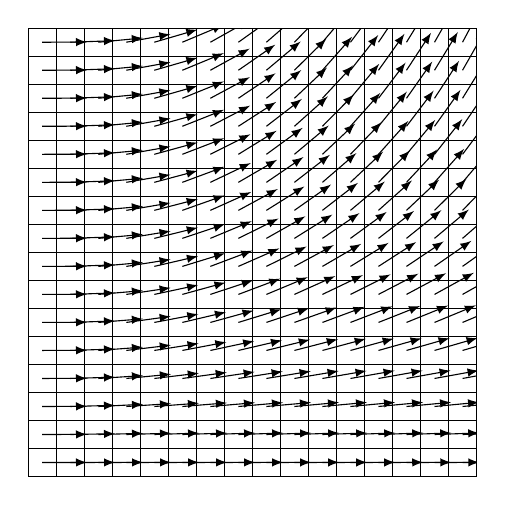
\begin{tikzpicture}
			\begin{axis}[dominantorientationaxis]
				\addplot3[dominantorientationvectors] {0};
			\end{axis}
		\end{tikzpicture}
		\caption{First subfigure} \label{fig:1a}
	\end{subfigure}
	\begin{subfigure}{\siftwidth}
		\centering
		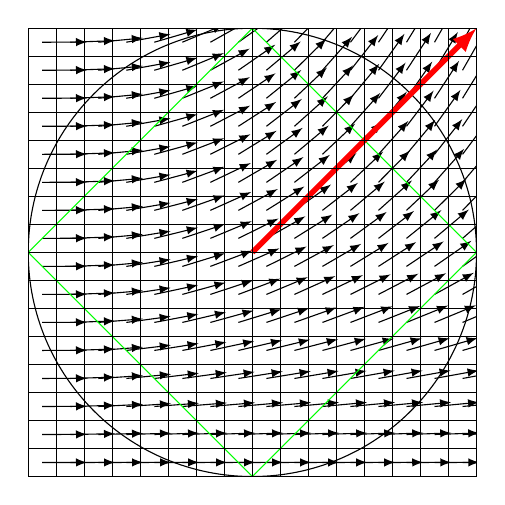
\begin{tikzpicture}[]
			\begin{axis}[dominantorientationaxis]
				\addplot3[dominantorientationvectors] {0};
				\draw (0.5, 0.5) circle [blue, radius=.5];
                \pic[rotate around={45:(0.5,0.5)}] {greensquare=.1464/.1464/.707};
				\draw[line width=2pt,red,-latex](.5,.5)--(1,1);
			\end{axis}
		\end{tikzpicture}
		\caption{First subfigure} \label{fig:1b}
	\end{subfigure}
	\vskip\baselineskip
	\begin{subfigure}{\siftwidth}
		\centering
		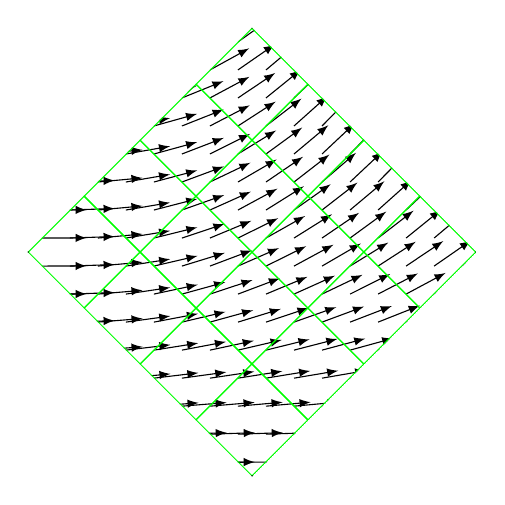
\begin{tikzpicture}[rotate=-45,transform shape]
			\clip[](2.04,2) rectangle (6.07,6.03);
			\begin{axis}[dominantorientationaxis, rotate around={45:(.5,.5)}, grid=none]
				\addplot3[dominantorientationvectors] {0};
				\pic[] {subgradbins};
			\end{axis}
		\end{tikzpicture}
		\caption{First subfigure} \label{fig:1c}
	\end{subfigure}
	\begin{subfigure}{\siftwidth}
		\centering
		\begin{tikzpicture}
			\coordinate (origin) at (0,0);
			\pgfmathtruncatemacro{\kmax}{div(3.0,1.0)}
			\begin{scope}[rotate=-45,transform shape,local bounding box=scope1]
				\foreach \i [evaluate=\i as \x using \i*1.0] in {0,...,\kmax}{
						\foreach \j [evaluate=\j as \x using \j*1.0] in {0,...,\kmax}{
								\pic {greensquare=\i/\j/1.0};
								\pgfmathtruncatemacro{\n}{\i*4+\j};
								\pic {randomedgehistogram=\i/\j};
							}
					}
			\end{scope}
			\begin{scope}[shift={($(scope1.south)-(0,1cm)$)}]
				\matrix (A) [matrix of math nodes, nodes={array, anchor=center}, column sep=-\pgflinewidth]
				{d_0,\dots,d_7 & d_8,\dots,d_{15} & \cdots\cdots\cdots & d_{120},\dots,d_{127} \\};
				\draw[decorate,decoration={brace, amplitude=10pt, raise=5pt, mirror}]
				(A-1-1.south west) to node[black,midway,below= 15pt] {$16 \times 8$ entries} (A-1-4.south east);%
				\path[-latex,red,thick] (hist-00) edge [] (A-1-1);
				\path[-latex,red,thick] (hist-10) edge [] (A-1-2);
				\path[-latex,red,thick] (hist-20) edge [] (A-1-3);
				\path[-latex,red,thick] (hist-30) edge [] (A-1-3);
				\foreach \i in {1,...,2}{
						\foreach \j in {0,...,3}{
								\path[-latex,red,thick] (hist-\j\i) edge [] (A-1-3);
							}
					}
				\path[-latex,red,thick] (hist-03) edge [] (A-1-3);
				\path[-latex,red,thick] (hist-13) edge [] (A-1-3);
				\path[-latex,red,thick] (hist-23) edge [] (A-1-3);
				\path[-latex,red,thick] (hist-33) edge [] (A-1-4);
			\end{scope}
		\end{tikzpicture}
		\begin{tikzpicture}

		\end{tikzpicture}
		\begin{tikzpicture}[overlay]
		\end{tikzpicture}
		\caption{First subfigure} \label{fig:1d}
	\end{subfigure}
	%	\caption{A figure that contains three subfigures} \label{fig:1}
\end{figure*}

